\setcounter{section}{0}
\setcounter{subsubsection}{0}
\setcounter{ex}{0}
\setcounter{bt}{0}
 
\subsection{ĐỀ SỐ 2}
\subsubsection{Bài tập trắc nghiệm bốn phương án lựa chọn}
\Opensolutionfile{ans}[ans/ans-1]
\begin{ex}%[BÀI GIẢNG ĐỢT 3, Huỳnh Đức Vũ]%[1D2N1-2]
	Cho dãy số $(u_n)$ với $u_n=3^n$. Số hạng thứ $n+1$ là
	\choice
	{$u_{n+1}=3^n+3$}
	{\True $u_{n+1}=3\cdot 3^n$}
	{$u_{n+1}=3^n+1$}
	{$u_{n+1}=3(n+1)$}
	\loigiai{
		Ta có $u_{n+1}=3^{n+1}=3\cdot 3^n$.\\
		Vậy số hạng thứ $n+1$ là $u_{n+1}=3\cdot 3^n$.
	}
\end{ex}
\begin{ex}%[BÀI GIẢNG ĐỢT 3, Huỳnh Đức Vũ]%[1D2N1-2]
	Cho dãy số $(u_n)$ thỏa mãn $\heva{&u_1=4\\&u_{n+1}=u_n+n}$. Năm số hạng đầu của dãy số là
	\choice
	{$4,\,5,\,6,\,7,\,8$}
	{$4,\,16,\,32,\,64,\,128$}
	{$4,\,6,\,9,\,13,\,18$}
	{\True $4,\,5,\,7,\,10,\,14$}
	\loigiai{
		Ta có
		\begin{eqnarray*}
			u_2&=&u_1+1=5;\\
			u_3&=&u_2+2=7; \\
			u_4&=&u_3+3=10; \\
			u_5&=&u_4+4=14.
		\end{eqnarray*}
		Vậy năm số hạng đầu của dãy số là	$4,\,5,\,7,\,10,\,14$.
	}
\end{ex}
\begin{ex}%[BÀI GIẢNG ĐỢT 3, Huỳnh Đức Vũ]%[1D2N1-2]
	Cho dãy số $(u_n)$ xác định bởi $\heva{&u_1=-3  \\& u_n=\dfrac{1}{2}u_{n-1}+1}$ với $n\in \mathbb{N}^*,\,n\ge 2$. Số hạng thứ $4$ của dãy số đã cho là
	\choice
	{$u_4=\dfrac{1}{2}$}
	{$u_4=1$}
	{\True $u_4=\dfrac{11}{8}$}
	{$u_4=\dfrac{5}{88}$}
	\loigiai{
		Ta có
		\begin{eqnarray*}
			u_2&=&\dfrac{1}{2}u_1+1=\dfrac{1}{2}\left(-3 \right)+1=\dfrac{-1}{2};\\
			u_3&=&\dfrac{1}{2}u_2+1=\dfrac{1}{2}.\dfrac{-1}{2}+1=\dfrac{3}{4};\\
			u_4&=&\dfrac{1}{2}{u_3}+1=\dfrac{1}{2}.\dfrac{3}{4}+1=\dfrac{11}{8}.
		\end{eqnarray*}
		Vậy số hạng thứ $4$ của dãy số đã cho là $u_4=\dfrac{11}{8}$.
	}
\end{ex}
\begin{ex}%[BÀI GIẢNG ĐỢT 3, Huỳnh Đức Vũ]%[1D2H1-5]
	Cho dãy số $(u_n)$ với $u_n=\dfrac{1}{n+2}$. Trong các mệnh đề dưới đây, mệnh đề nào đúng?
	\choice
	{\True Dãy số $(u_n)$ là dãy số giảm và bị chặn}
	{Dãy số $(u_n)$ là dãy số tăng và bị chặn trên}
	{Dãy số $(u_n)$ là dãy số giảm và không bị chặn dưới}
	{Dãy số $(u_n)$ là dãy số tăng và không bị chặn trên}
	\loigiai{
		Ta có $$u_{n+1}=\dfrac{1}{(n+1)+2}=\dfrac{1}{n+3}<\dfrac{1}{n+2}=u_n.$$ 
		$\Rightarrow u_{n+1}<u_n,\,\forall n\in \mathbb{N}^*$.\\
		Suy ra dãy số $(u_n)$ là dãy số giảm.\\
		Với $\forall n\in \mathbb{N}^*$ ta có $0<\dfrac{1}{n+2}<1$ hay $0<u_n<1$.\\
		Suy ra dãy số $u_n$ là dãy số bị chặn.\\
		Vậy dãy số $u_n$ là dãy số giảm và bị chặn.
	}
\end{ex}
\begin{ex}%[BÀI GIẢNG ĐỢT 3, Huỳnh Đức Vũ]%[1D2H2-2]
	Cho cấp số cộng $(u_n)$ biết $u_5=5$, $u_{10}=15$. Số hạng thứ $7$ là
	\choice
	{$u_7=12$}
	{$u_7=8$}
	{$u_7=7$}
	{\True $u_7=9$}
	\loigiai{
		Cấp số cộng $(u_n)$ có 
		$$\heva{&u_5=5\\&u_{10}=15} \Leftrightarrow \heva{&u_1+4d=5\\&u_1+9d=15} \Leftrightarrow \heva{&u_1=-3\\&d=2.}$$
		Vậy số hạng thứ $7$ là $u_7=u_1+6d=-3+6\cdot 2=9$.
		
	}
\end{ex}
\begin{ex}%[BÀI GIẢNG ĐỢT 3, Huỳnh Đức Vũ]%[1D2H2-5]
	Biết bốn số $5$; $x$; $15$; $y$ theo thứ tự đó lập thành cấp số cộng. Giá trị của biểu thức $3x+2y$ bằng
	\choice
	{$50$}
	{\True $70$}
	{$30$}
	{$80$}
	\loigiai{
		Do $5$; $x$; $15$; $y$ theo thứ tự đó lập thành cấp số cộng nên $x=\dfrac{5+15}{2}=10$.\\
		Ngoài ra $x+y=2\cdot 15$ nên $y=30-x=30-10=20$.\\
		Vậy $3x+2y=70$.}
\end{ex}
\begin{ex}%[BÀI GIẢNG ĐỢT 3, Huỳnh Đức Vũ]%[1D2H2-2]
	Bốn số tạo thành một cấp số cộng có tổng bằng 32 và tổng các bình phương của chúng bằng 336. Tích của bốn số đó là
	\choice
	{$5760$}
	{$15120$}
	{$1920$}
	{\True $1680$}
	\loigiai{Gọi bốn số cần tìm là $a$, $a+d$, $a+2d$, $a+3d$. Từ giả thiết ta suy ra
		\begin{align*}
			&\heva{&a+a+d+a+2d+a+3d=32\\&a^2+(a+d)^2+(a+2d)^2+(a+3d)^2=336}\Leftrightarrow\heva{&2a=16-3d\\&4a^2+12ad+14d^2=336}\\
			\Leftrightarrow&\heva{&2a=16-3d\\&(16-3d)^2+6d(16-3d)+14d^2=336}\Leftrightarrow\heva{&\hoac{&d=4\\&d=-4}\\&2a=16-3d}\Leftrightarrow\hoac{&\heva{&d=4\\&a=2}\\&\heva{&d=-4\\&a=14.}}
		\end{align*}
		Vậy suy ra bốn số đó là $2$, $6$, $10$, $14$, nên tích của chúng là $P=1680$.}
\end{ex}
\begin{ex}%[BÀI GIẢNG ĐỢT 3, Huỳnh Đức Vũ]%[1D2H2-2]
	Cho cấp số cộng $(u_n)$ biết $u_5=18$ và $4S_n=S_{2n}$. Số hạng đầu $u_1$ và công sai $d$ của cấp số cộng là
	\choice
	{$u_1=3$, $d=2$}
	{$u_1=2$, $d=3$}
	{$u_1=2$, $d=2$}
	{\True $u_1=2$, $d=4$}   
	\loigiai{
		Từ giả thiết ta có hệ 
		\begin{eqnarray*}
			&&\heva {&u_5=18\\&4S_n=S_{2n}}\\
			&\Leftrightarrow & \heva {&u_1+4d=18\\&4n\cdot \dfrac{u_1+u_n}{2}=2n\cdot \dfrac{u_1+u_{2n}}{2}}\\&\Leftrightarrow& \heva {&u_1+4d=18\\&2(u_1+u_n)=u_1+u_{2n}}\\
			&\Leftrightarrow & \heva {&u_1+4d=18\\&2\left[2u_1+(n-1)d\right]=2u_1+(2n-1)d}\\&\Leftrightarrow& \heva {&u_1+4d=18\\&2u_1-d=0}\\&\Leftrightarrow& \heva {&u_1=2\\&d=4.}
		\end{eqnarray*}
	} 
\end{ex}
\begin{ex}%[BÀI GIẢNG ĐỢT 3, Huỳnh Đức Vũ]%[1D2H3-2]%Câu 8 
	Một tam giác có số đo các góc lập thành cấp số nhân có công bội $q=2$. Số đo các góc của tam giác đó lần lượt là 
	\choice
	{$\dfrac{\pi }{6}$; $\dfrac{\pi }{3}$; $\dfrac{\pi }{2}$}
	{$\dfrac{\pi }{5}$; $\dfrac{2\pi }{5}$; $\dfrac{4\pi }{5}$}
	{$\dfrac{\pi }{6}$; $\dfrac{2\pi }{6}$; $\dfrac{4\pi }{6}$}
	{\True $\dfrac{\pi }{7}$; $\dfrac{2\pi }{7}$; $\dfrac{4\pi }{7}$}
	\loigiai{
		Giả sử tam giác $ABC$ có ba góc theo thứ tự lập thành cấp số nhân với công bội $q=2$.\\
		Ta có $B=2A$; $C=4A$.\hfill $(1)$\\
		Mà $A+B+C=\pi$. \hfill $(2)$\\
		Từ $(1)$ và $(2)$ suy ra $A=\dfrac{\pi}{7}$.\\
		Vậy số đo các góc của tam giác đó lần lượt là $\dfrac{\pi }{7}$; $\dfrac{2\pi }{7}$; $\dfrac{4\pi }{7}$.}
\end{ex}

\begin{ex}%[BÀI GIẢNG ĐỢT 3, Huỳnh Đức Vũ]%Câu 1%[1D2N3-2]
	Trong các dãy số sau, dãy số nào là cấp số nhân?
	\choice
	{$\heva{
			& {u_1}=\dfrac{1}{2} \\ 
			& u_{n+1}=u_n^2 \\ 
		} $}
	{$u_{n+1}=n{u_n}$}
	{\True $\heva{
			& {u_1}=2 \\ 
			& u_{n+1}=-5{u_n} \\ 
		} $}
	{$u_{n+1}=u_{n+1}-3$}
	\loigiai{
		Ta có $\heva{&
			{u_1}=2 \\&
			u_{n+1}=-5{u_n}}\Rightarrow \dfrac{u_{n+1}}{u_n}=-5, \;\forall n \in \mathbb{N^*}$.\\
		$\Rightarrow \left( {u_n} \right)$ là cấp số nhân có số hạng đầu ${u_1}=2$ và công bội $q=-5$.}
\end{ex}
\begin{ex}%[BÀI GIẢNG ĐỢT 3, Huỳnh Đức Vũ]%Câu 2%[1D2N3-2]
	Cho các cấp số nhân với $u_1=\dfrac{-1}{2};{u_7}=-32$. Công bội của cấp số nhân là
	\choice
	{$\pm \dfrac{1}{2}$}
	{ $\pm 4$}
	{\True$\pm 2$}
	{$\pm 1$}
	\loigiai{
		Ta có $u_7=u_1q^6\Rightarrow -32=-\dfrac{1}{2}q^6\Rightarrow q=\pm 2$.}
\end{ex}
\begin{ex} %[1D2H3-2]
	Cho cấp số nhân $(u_n)$ có $u_1=-1$, công bội $q=-\dfrac{1}{10}$. Khi đó $\dfrac{1}{10^{2017}}$ là số hạng thứ
	\choice
	{$2016$}
	{$2017$}
	{\True $2018$}
	{$2019$}
	\loigiai{
		Ta có số hạng tổng quát của dãy số là $u_n=u_1\cdot q^{n-1}=\left(-1\right)\cdot \left(-\dfrac{1}{10}\right)^{n-1}$.\\
		Giả sử $\dfrac{1}{10^{2017}}$ là số hạng thứ $n$ của cấp số nhân, ta có $$u_n=\dfrac{1}{10^{2017}}  \Leftrightarrow (-1)\cdot \left(-\dfrac{1}{10}\right)^{(n-1)}=\dfrac{1}{10^{2017}}\Leftrightarrow n=2018.$$	}
\end{ex}
\begin{ex}%[BÀI GIẢNG ĐỢT 3, Huỳnh Đức Vũ]%[1D2H3-4]
	Cho cấp số nhân với $u_1=3$, $q=-\dfrac{1}{2}$. Số $222$ là số hạng thứ mấy của cấp số nhân?
	\choice
	{Số hạng thứ $11$}
	{Số hạng thứ $9$}
	{Số hạng thứ $12$}
	{\True Không thuộc cấp số nhân}
	\loigiai{
		Giả sử số $222$ là số hạng thứ $n$.\\
		Ta có $u_n=u_1{q^{n-1}}\Leftrightarrow 222=3\cdot {{\left( -\dfrac{1}{2} \right)}^{n-1}}\Leftrightarrow {{\left( -\dfrac{1}{2} \right)}^{n-1}}=74$ (không tồn tại $n\in \mathbb{N}$ thỏa mãn).\\
		Vậy $222$ không là số hạng của cấp số nhân.}
\end{ex}
\begin{ex}%[BÀI GIẢNG ĐỢT 3, Huỳnh Đức Vũ]%Câu 54%[1D2V3-6]
	Cho dãy số $\left( {u_n} \right)$ xác định bởi $u_1=\dfrac{1}{3}$ và $u_{n+1}=\dfrac{n+1}{3n}\cdot {u_n}$. Giá trị của tổng \\ $S=u_1+\dfrac{u_2}{2}+\dfrac{u_3}{3}+\cdots+\dfrac{{u_{10}}}{10}$ là
	\choice
	{$\dfrac{3280}{6561}$}
	{\True $\dfrac{29524}{59049}$}
	{$\dfrac{25942}{59049}$}
	{$\dfrac{1}{243}$}
	\loigiai{
		Theo đề ta có $$u_{n+1}=\dfrac{n+1}{3n}\cdot	 {u_n}\Leftrightarrow \dfrac{u_{n+1}}{n+1}=\dfrac{1}{3}\dfrac{u_n}{n}.$$
		Mà $u_1=\dfrac{1}{3}$ nên $\dfrac{u_2}{2}=\dfrac{1}{3}\cdot \dfrac{1}{3}={{\left(\dfrac{1}{3} \right)}^2};\dfrac{u_3}{3}=\dfrac{1}{3}\cdot {{\left( \dfrac{1}{3} \right)}^2}={{\left( \dfrac{1}{3} \right)}^3};\ldots;\dfrac{{u_{10}}}{10}={{\left( \dfrac{1}{3} \right)}^{10}}$.\\
		Do đó dãy $\left( \dfrac{u_n}{n} \right)$ là một cấp số nhân có số hạng đầu $u_1=\dfrac{1}{3}$, công bội $q=\dfrac{1}{3}$.\\
		Khi đó $S=u_1+\dfrac{u_2}{2}+\dfrac{u_3}{3}+\cdots+\dfrac{{u_{10}}}{10}=\dfrac{{3^{10}}-1}{{{2\cdot 3}^{10}}}=\dfrac{59048}{2\cdot 3^{10}}=\dfrac{29524}{59049}$.}
\end{ex}
\begin{ex}%[BÀI GIẢNG ĐỢT 3, Huỳnh Đức Vũ]%Câu 55%[1D2H3-4]
	Cho cấp số nhân $\left( {u_n} \right)$ có $u_n=24$; $\dfrac{{u_4}}{{u_{11}}}=16384$. Số hạng thứ $17$ của cấp số nhân là
	\choice
	{$\dfrac{3}{67108864}$}
	{$\dfrac{3}{268435456}$}
	{\True $\dfrac{3}{536870912}$}
	{$\dfrac{3}{214783648}$}
	\loigiai{
		Từ $\dfrac{{u_4}}{{u_{11}}}=16384\Leftrightarrow \dfrac{1}{q^7}=16384\Leftrightarrow q^7={{\left( \dfrac{1}{4} \right)}^7}\Leftrightarrow q=\dfrac{1}{4}$.\\
		Ta có $u_n=24$ tương ứng khi $n = 1$.\\
		Số hạng thứ $17$ của cấp số nhân là ${u_{17}}=24\cdot{{\left( \dfrac{1}{4} \right)}^{16}}=\dfrac{3}{536870912}$.}
\end{ex}

\begin{ex} %[1D2V3-2]
	Một cái tháp có $11$ tầng. Diện tích của mặt sàn tầng $2$ bằng nửa diện tích của mặt đáy tháp và diện tích của mặt sàn mỗi tầng bằng nửa diện tích của mặt sàn mỗi tầng ngay bên dưới. Biết mặt đáy tháp có diện tích là $12 288m^2$. Tính diện tích của mặt sàn tầng trên cùng của tháp theo đơn vị mét vuông.
	\choice{\True$12\mathrm{m^2}$}{$24\mathrm{m^2}$}{$6\mathrm{m^2}$}{$48\mathrm{m^2}$}
	\loigiai{
		Do diện tích của mặt sàn tính từ tầng một lập thành một cấp số nhân với $u_2=\dfrac{1}{2}.12288=6144$ và $q=\dfrac{1}{2}$.\\
		Ta có $\heva{u_2&=6144 \\ q&=\dfrac{1}{2}}  \Leftrightarrow \heva{u_1&=12288 \\ q&=\dfrac{1}{2}}$.\\
		Ta có $u_{11}=u_1.q^{10}=12288.\dfrac{1}{12^{10}}=12m^2$.\\
		Vậy diện tích của mặt sàn tầng trên cùng là	$12\mathrm{m^2}$.
	}
\end{ex}
\Closesolutionfile{ans}
\indapan{10}{ans/ans-1}
\subsubsection{Bài tập trắc nghiệm đúng sai}
\Opensolutionfile{ans}[ans/ans-2]
\setcounter{ex}{0}
\begin{ex}%[BÀI GIẢNG ĐỢT 3, Huỳnh Đức Vũ]%[1D2V3-8]%Câu 1
	Chị Mai gửi tiền tiết kiệm vào ngân hàng theo thể thức lãi kép như sau: Lần đầu chị gửi $100$ triệu đồng. Sau đó, cứ hết $1$ tháng chị lại gửi thêm vào ngân hàng $6$ triệu đồng. Biết lãi suất của ngân hàng là $0{,}5\%$ một tháng. Gọi $P_n$ (triệu đồng) là số tiền chị có trong ngân hàng sau $n$ tháng.
	\choiceTF[t]
	{\True Số tiền chị có trong ngân hàng sau $1$ tháng là $106\,500\,000$ đồng}
	{Số tiền chị có trong ngân hàng sau $3$ tháng là $119\,500\,000$ đồng}
	{\True Số tiền lãi chị có được trong ngân hàng sau $4$ tháng là $20\,195\,656$ đồng}
	{\True Dự đoán công thức của $P_n$ tính theo $n$ là $P_n=100\cdot{1{,}005^n}+\dfrac{6\cdot{1{,}005^n}-6}{0{,}005}$}
	\loigiai{
\begin{itemchoice}
\itemch Đúng.\\Số tiền lãi chị Mai thu được sau tháng thứ $1$ là $100000000\cdot 0{,}5\%=500000$ đồng.\\
			Do đó $P_1=100\,000\,000+500\,000+6\,000\,000=106\,500\,000$ đồng.
\itemch Sai.\\Số tiền chị có trong ngân hàng sau tháng thứ $2$ là\\
			$P_2=P_1+P_1\cdot 0{,}5\%+6\,000\,000=113\,032\,500$ đồng.\\
			Số tiền chị có trong ngân hàng sau tháng thứ $3$ là\\
			$P_3=P_2+P_2\cdot 0{,}5\%+6=119\,597\,662$ đồng.
\itemch Đúng.\\Số tiền chị có trong ngân hàng sau tháng thứ $4$ là\\
			$P_4=P_3+P_3\cdot 0{,}5\%+6=120\,195\,656$ đồng.\\
			Số tiền lãi chị có được trong ngân hàng sau $4$ tháng là\\
			$120\,195\,656-100\,000\,000=20\,195\,656$ đồng.
\itemch Đúng.\\Ta chọn đơn vị là triệu đồng và xét bài toán tổng quát: Số tiền ban đầu là $T$ triệu đồng với lãi suất hàng tháng là $r$ và mỗi tháng gửi thêm $a$ triệu đồng thì số tiền trong tài khoản sau tháng thứ $n$ là $P_n$ triệu đồng. Số tiền lãi sau tháng thứ $n$ được tính là $P_n\cdot r$ nên ta có
\begin{itemize}
\item $P_1=T+T\cdot r+a=T(1+r)+a=T(1+r)+\dfrac{a{(1+r)^1}-a}{r}$;
\item $P_2=P_1+P_1\cdot r+a=T{(1+r)^2}+(r+1)\cdot\dfrac{a{(1+r)^1}-a}{r}+a=T{(1+r)^2}+\dfrac{a{(1+r)^2}-a}{r}$;
\item $P_3=P_2+P_2\cdot r+a=T{(1+r)^3}+(r+1)\cdot\dfrac{a{(1+r)^2}-a}{r}+a=T{(1+r)^3}+\dfrac{a{(1+r)^3}-a}{r}$. \\
$\ldots$
\item Cứ tiếp tục như vậy thì ta dự đoán công thức tổng quát của $P_n$ là\\
			$P_n=T{(1+r)^n}+\dfrac{a{(1+r)^n}-a}{r}.$		
\end{itemize}
Thay số $T=100$, $r=0{,}5\%=0{,}005$ và $a=6$ ta thu được\\
$$P_n=100\cdot{1{,}05^n}+\dfrac{6\cdot{1{,}005^n}-6}{0{,}005}.$$
	\end{itemchoice}	
	}
	\end{ex}
	
	\begin{ex}%[BÀI GIẢNG ĐỢT 3, Huỳnh Đức Vũ]%[1D2V3-8]%Câu 2
		Một sinh viên sau khi ra trường và xin vào làm cho một trung tâm với mức lương khởi điểm là 100 triệu đồng một năm. Cứ sau mỗi năm, trung tâm trả thêm cho sinh viên $ 15$ triệu đồng. Gọi $u_n$ (triệu đồng) là số tiền lương mà sinh viên đó nhận được ở năm thứ $ n$. Hỏi các mệnh đề sau đúng hay sai?
		\choiceTF[t]
		{\True Số tiền lương sinh viên nhận được ở năm thứ hai là $ 115$ triệu đồng}
		{Số tiền lương sinh viên nhận được ở năm thứ $10$ là $ 300$ triệu đồng}
		{Dãy số $\left(u_n\right)$ là cấp số cộng có $u_1=120$ và công sai $ d=20$}
		{Giả sử, mỗi năm bạn sinh viên chi tiêu tiết kiệm hết $70$ triệu đồng. Vậy sau $12$ năm thì sinh viên đó mua được căn chung cư $2$ tỉ đồng}
		\loigiai{
			Ta thấy, số tiền lương năm sau hơn năm trước $ 15$ triệu đồng nên $\left(u_n\right)$ là cấp số cộng có $u_1=100$ và công sai $ d=15$.\\ Do đó $u_n=u_1+\left(n-1\right)d=100+\left(n-1\right)\cdot 15=15n+85$.
	\begin{itemchoice}
	\itemch Đúng.\\
			Số tiền lương sinh viên nhận được ở năm thứ hai là\\
				$u_2=u_1+d=100+15=115$ (triệu đồng).\\
				suy ra mệnh đúng.
	\itemch Sai.\\
	Số tiền lương sinh viên nhận được ở năm thứ $10$ là\\
				$u_{10}=u_1+9d=15.10+85=235$(triệu đồng).\\
				Suy ra mệnh sai.
	\itemch Sai.\\Dãy số $\left(u_n\right)$ là cấp số cộng có $u_1=100$ và công sai $ d=15$ suy ra mệnh đề sai.
	\itemch Sai.\\Tổng số tiền bạn sinh viên tiết kiệm được sau $ n$ năm là $$ S=\dfrac{n}{2}\left[2u_1+\left(n-1\right)d\right]-70n=\dfrac{n}{2}\left[2\cdot  100+\left(n-1\right)\cdot 15\right]-70n=\dfrac{15}{2}{n^2}+\dfrac{45}{2}n\,\text{(triệu đồng)}.$$\\
				Ta có $ S\ge 2000$$\Leftrightarrow\dfrac{15}{2}{n^2}+\dfrac{45}{2}n-2000\ge 0\Leftrightarrow\hoac{
					& n\ge 14{,}9\\ 
					& n\le-17{,}9.}\Leftrightarrow n \ge 15$.\\
				Vậy sau $15$ năm thì sinh viên đó có thể mua được chung cư với số tiền $2$ tỉ đồng.\\
				Suy ra mệnh đề này là mệnh đề sai.
	\end{itemchoice}
		}
		\end{ex}
		
		\begin{ex}%[BÀI GIẢNG ĐỢT 3, Huỳnh Đức Vũ]%[1D2V3-8]%Câu 3
			Bạn Xuân có một cái lọ. Ngày thứ nhất bạn bỏ vào lọ $1$ viên kẹo, ngày thứ hai bạn bỏ vào $2$ viên kẹo, ngày thứ ba bạn bỏ vào $4$ viên kẹo Biết sau khi bỏ hết số kẹo ở ngày thứ $12$ thì lọ đầy. Các mệnh đề sau đây đúng hay sai?
			\choiceTF[t]
			{Ngày thứ ba số kẹo trong lọ là $4$ viên}
			{\True Ngày thứ tư số kẹo trong lọ là $15$ viên}
			{\True Số kẹo khi lọ đầy là $4095$ viên}
			{Đến ngày thứ $9$ số kẹo trong lọ chiếm $\dfrac{1}{4}$ lọ?}
			\loigiai{
	\begin{itemchoice}
	\itemch Sai.\\
	Nhận xét: Quá trình bỏ viên kẹo ngày qua ngày của bạn Xuân theo quy tắc là một cấp số nhân với số hạng đầu và công bội lần lượt là $u_1=1,q=2$.\\
					Ngày thứ ba số kẹo trong lọ là $ 1+2+4=7$ viên. Suy ra mệnh đề sai.
	\itemch Đúng.\\Ngày thứ tư số kẹo trong lọ là $ 1+2+4+8=15$ viên. Suy ra mệnh đề đúng.
	\itemch Đúng.\\ Quá trình bỏ viên kẹo ngày qua ngày của bạn Xuân theo quy tắc là một cấp số nhân với số hạng đầu và công bội lần lượt là $u_1=1$, $q=2$.\\
					Gọi tổng số kẹo mà bạn ấy bỏ vào lọ là $ S$. Do đến ngày thứ $12$ lọ đầy nên ta có công thức sau\\
					$S_{12}=u_1+u_2+\ldots+u_{12}=1+2+2^2+\ldots+2^{11}=\dfrac{2^{12}-1}{2-1}=4095.$ Suy ra mệnh đề đúng.
	\itemch Sai.\\Quá trình bỏ viên kẹo ngày qua ngày của bạn Xuân theo quy tắc là một cấp số nhân với số hạng đầu và công bội lần lượt là $u_1=1,q=2$.\\
					Gọi tổng số kẹo mà bạn ấy bỏ vào lọ là $ S,$ do đến ngày thứ $12$ lọ đầy nên ta có công thức sau\\
					$S_{12}=u_1+u_2+\ldots+u_{12}=1+2+2^2+..+2^{11}=\dfrac{2^{12}-1}{2-1}=4095.$\\
					Để số kẹo chiếm $\dfrac{1}{4}$ lọ thì cần $\dfrac{4095}{4}$ viên kẹo.\\
					Gọi $ n$ là số ngày, ta có $S_n=u_1+u_2+\ldots+u_n=1+2+\ldots+2^{n-1}=2^n-1$.\\
					Mà $S_n=\dfrac{4095}{4}\Leftrightarrow n\approx 10$. Suy ra mệnh đề sai.
	\end{itemchoice}		
			}
			\end{ex}
			
			\begin{ex}%[BÀI GIẢNG ĐỢT 3, Huỳnh Đức Vũ]%[1D2V3-8]%Câu 4
				Bạn Ngọc thả một quả bóng cao su từ độ cao $ 20m$ m so với mặt đất, mỗi lần chạm đất quả bóng lại nảy lên một độ cao bằng bốn phần năm độ cao lần rơi trước. Biết rằng quả bóng luôn chuyển động vuông góc với mặt đất. Các mệnh đề sau đây đúng hay sai?
				\choiceTF[t]
				{Quãng đường quả bóng rơi xuống từ lúc thả đến lúc chạm đất lần đầu là $ 16$ m}
				{Quả bóng chạm đất lần đầu nảy lên với độ cao là $ 36$ m}
				{\True Tổng quãng đường quả bóng đã di chuyển được từ lúc thả bóng cho đến lúc bóng chạm đất lần hai là $ 52$ m}
			{\True Tổng quãng đường quả bóng đã di chuyển được (từ lúc thả bóng cho đến lúc bóng không nảy nữa) là $ 180(m)$}
			\loigiai{
	\begin{itemchoice}
	\itemch Sai.\\
		Quãng đường quả bóng rơi xuống từ lúc thả đến lúc chạm đất lần đầu là $ 20(m)$. Suy ra mệnh đề sai.
	\itemch Sai.\\Vì mỗi lần chạm đất quả bóng lại nảy lên một độ cao bằng bốn phần năm độ cao lần rơi trước, nên quả bóng chạm đất lần đầu nảy lên với độ cao là $\dfrac{4}{5}\text{20=16}$ m. Suy ra mệnh đề sai.
	\itemch Đúng.\\
					Quãng đường quả bóng rơi xuống từ lúc thả đến lúc chạm đất lần đầu là $ 20$ m.\\
					Quãng đường quả bóng nảy lên khi chạm đất lần đầu là $ 16$ m.\\
					Quãng đường quả bóng rơi xuống chạm đất lần hai là $ 16$ m.\\
					Tổng quãng đường quả bóng đã di chuyển được từ lúc thả bóng cho đến lúc bóng chạm đất lần hai là $ 20+16+16=52$ m.\\
					Suy ra mệnh đề đúng.
	\itemch Đúng.\\Ta có quãng đường bóng bay bằng tổng quãng đường bóng nảy lên và quãng đường bóng rơi xuống.\\
					Vì mỗi lần bóng nảy lên bằng $\dfrac{4}{5}$ lần nảy trước nên ta có tổng quãng đường bóng nảy lên là $S_1=20.\dfrac{4}{5}+20.\left(\dfrac{4}{5}\right)^2+20.\left(\dfrac{4}{5}\right)^3+\ldots+20.\left(\dfrac{4}{5}\right)^n+\ldots$\\
					Đây là tổng của cấp số nhân lùi vô hạn có số hạng đầu $u_1=20.\dfrac{4}{5}=16$ và công bội $ q=\dfrac{4}{5}$.\\
					Suy ra $S_1=\dfrac{16}{1-\dfrac{4}{5}}=80$.\\
					Tổng quãng đường bóng rơi xuống bằng khoảng cách độ cao ban đầu và tổng quãng đường bóng nảy lên nên là $S_2=20+20.\left(\dfrac{4}{5}\right)+20.\left(\dfrac{4}{5}\right)^2+\ldots+20.\left(\dfrac{4}{5}\right)^n+\ldots$\\
					Đây là tổng của cấp số nhân lùi vô hạn với số hạng đầu $u_1=20$ và công bội $ q=\dfrac{4}{5}$.\\
					Suy ra $S_2=\dfrac{20}{1-\dfrac{4}{5}}=100$.\\
					Vậy tổng quãng đường bóng bay là $ S=S_1+S_2=180$. Suy ra mệnh đề đúng.
	\end{itemchoice}
			}
			\end{ex}
\Closesolutionfile{ans}
\indapan{4}{ans/ans-2}
\subsubsection{Bài tập trắc nghiệm trả lời ngắn}
\Opensolutionfile{ans}[ans/ans-3]
\setcounter{ex}{0}
\begin{ex}%[BÀI GIẢNG ĐỢT 3, Huỳnh Đức Vũ]%[1D2V3-6]
Cho một cấp số cộng $(u_n)$ có $S_6 = 18$ và $S_{10} = 110$. Tính $S_{20}$.
\shortans{$620$}
\loigiai{Giả sử cấp số cộng $(u_n)$ có số hạng đầu là $u_1$ và công sai là $d$.\\
Ta có $S_6 = 6u_1 + \dfrac{6 \cdot 5}{2}d \Leftrightarrow 6u_1 + 15d = 18$. \quad (1)\\
$S_{10} = 10u_1 + \dfrac{10 \cdot 9}{2}d \Leftrightarrow 10u_1 + 45d = 110$. \quad (2)\\
Từ (1) và (2), ta có hệ phương trình $\heva{&6u_1 + 15d = 18\\&10u_1 + 45d = 110} \Leftrightarrow \heva{&u_1 = -7\\&d = 4.}$\\
					Khi đó $S_{20} = 20u_1 + \dfrac{20 \cdot 19}{2}d = 20 \cdot (-7) + 190 \cdot 4 = 620$.}
\end{ex}
\begin{ex}%[BÀI GIẢNG ĐỢT 3, Huỳnh Đức Vũ]%[1D2V3-6]%Câu 2
Cho cấp số cộng có số hạng tổng quát $u_n=5n-7$, biết tổng $n$ số hạng đầu của cấp số cộng là $S_n=817$. Tìm $n$.
\shortans{$19$}			
\loigiai{
Gọi $u_1$ là số hạng đầu của cấp số cộng $\left(u_n\right)$.\\
				Vì $u_n=5n-7$ nên $u_1=5.1-7=-2$.\\
				Áp dụng công thức $S_n=\dfrac{n\left(u_1+u_n\right)}{2}$, suy ra $817=\dfrac{n\left[-2+\left(5n-7\right)\right]}{2}$.\\
				Hay $5n^2-9n-1634=0\Leftrightarrow\hoac{
					& n=19\\ 
					& n=-\dfrac{86}{5}.}$\\
				Với điều kiện $n\in{\mathbb{N}^*}$, ta tìm được $n=19$.}
\end{ex}

\begin{ex}%[BÀI GIẢNG ĐỢT 3, Huỳnh Đức Vũ]%[1D2V3-6]%Câu 4
Cho cấp số nhân $\left(u_n\right)$, biết $u_1=2,\,\,u_2=-4$. Gọi $S_n$ là tổng $n$ số hạng đầu tiên của cấp số nhân đó, biết $S_n=1366$. Hỏi giá trị của $n$ bằng bao nhiêu?
\shortans{$11$}	
\loigiai{Theo bài ra, ta có $u_1=2,\,\,u_2=-4\Rightarrow q=\dfrac{u_2}{u_1}=-2$.\\
Áp dụng công thức tính tổng $n$ số hạng đầu tiên của cấp số nhân với $u_1=2,\,\,q=-2$, ta có\\
$S_n=u_1\dfrac{1-q^n}{1-q}=\dfrac{2}{3}.\left[1-\left(-2\right)^n\right]$.\\
Do $S_n=1366$ nên suy ra $\dfrac{2}{3}\left[1-\left(-2\right)^n\right]=1366\Leftrightarrow 1-\left(-2\right)^n=2049\Leftrightarrow n=11.$\\
Vậy giá trị của $n$ bằng $11$.}
\end{ex}
\begin{ex}%[BÀI GIẢNG ĐỢT 3, Huỳnh Đức Vũ]%[1D2V3-6]%Câu 5
Cho dãy cấp số nhân $\left(u_n\right)$ biết $\heva{
				&{u_3}-u_1=12\\ 
				&{u_6}-u_4=96}$. Tổng $S_7=u_1+u_2+u_3+u_4+u_5+u_6+u_7$ bằng?
\shortans{$508$}	
\loigiai{Ta có $\heva{
					&{u_3}-u_1=12\\ 
					&{u_6}-u_4=96}\Leftrightarrow\heva{
					&{u_1}{q^2}-u_1=12\\ 
					&{u_1}{q^5}-u_1q^3=96}\Leftrightarrow\heva{
					&{u_1}\left(q^2-1\right)=12\qquad(1)\\ 
					&{u_1}{q^3}\left(q^2-1\right)=96. \qquad(2)}$\\
				Lấy $(2)$ chia $(1)$ theo vế ta được $q^3=8\Rightarrow q=2$.\\
				Thay $q=2$ vào $(1)$ ta suy ra được $u_1=4$.\\
				Vậy $S_7=u_1.\dfrac{q^7-1}{q-1}=4.\dfrac{2^7-1}{2-1}=508$.}
\end{ex}
\begin{ex}%[BÀI GIẢNG ĐỢT 3, Huỳnh Đức Vũ]%[1D2V3-8]
	\immini{
		Cho hình vuông $ABCD$ có các cạnh bằng $a=10$ dm và có diện tích $S_1$.
		Nối $4$ trung điểm $A_1,B_1,C_1,D_1$ theo thứ tự của 4 cạnh $AB, BC, CD, DA$ 
		ta được hình vuông thứ hai có diện tích $S_2$. Tiếp tục làm như thế,
		ta được hình vuông thứ ba là $A_2$, $B_2$, $C_2$, $D_2$ có diện tích $S_3$,\ldots
		và cứ tiếp tục làm như thế, ta tính được các hình vuông lần lượt
		có diện tích có diện tích $S_4$, $S_5$, $\ldots$, $S_{100}$ (tham khảo hình vẽ bên).
		Tính tổng có diện tích $S=S_1+S_2+S_3+ \cdots +S_{100}$ (làm tròn đến hàng đơn vị).}{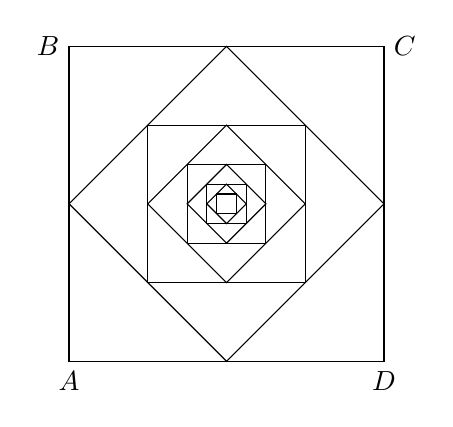
\begin{tikzpicture}
			\def\a{2} %cạnh hình vuông
			\def\t{.5} % tỷ lệ điểm cho vòng lặp tiếp
			\path
			(-\a,-\a) coordinate (A1)node[below]{$A$}
			(-\a,\a) coordinate (B1)node[left]{$B$}
			(\a,\a) coordinate (C1)node[right]{$C$}
			(\a,-\a) coordinate (D1)node[below]{$D$};
			\draw (A1)--(B1)--(C1)--(D1)--cycle;
			\foreach \i[count=\j from 2] in {1,...,8}
			\draw
			(barycentric cs:A\i=\t,B\i=1-\t) coordinate (A\j)--
			(barycentric cs:B\i=\t,C\i=1-\t) coordinate (B\j)--
			(barycentric cs:C\i=\t,D\i=1-\t) coordinate (C\j)--
			(barycentric cs:D\i=\t,A\i=1-\t) coordinate (D\j)--cycle
			;
	\end{tikzpicture}}
	\shortans{$200$}
	\loigiai{
		Ta có $S_1=a^2$; $S_2=\dfrac{1}{2}a^2$; $S_3=\dfrac{1}{4}a^2$, $\ldots$ \\
		Do đó $S_1$, $S_2$, $S_3$, $\ldots$, $S_{100}$ là cấp số nhân với số hạng đầu $u_1=S_1=a^2$ và công bội $q=\dfrac{1}{2}$.\\
		Suy ra $S=S_1+S_2+S_3+ \cdots +S_{100}=S_1 \cdot \dfrac{1-q^n}{1-q}=\dfrac{a^2(2^{100}-1)}{2^{99}}$.\\
	Thay $a=10$ ta được $S=\dfrac{100\cdot (2^{100}-1)}{2^{99}}\approx 200$ dm$^2$.}
\end{ex}
\begin{ex}%[BÀI GIẢNG ĐỢT 3, Huỳnh Đức Vũ]%[1D2V3-7]
	Ba số khác nhau có tổng bằng $114$ có thể coi là ba số hạng liên tiếp của một cấp số nhân hoặc coi là số hạng thứ nhất, thứ tư và thứ $25$ của $1$ cấp số cộng. Tính tổng các số đó.
\shortans{$114$}
\loigiai{ Gọi $3$ số cần tìm là $x$, $y$, $z$. Theo bài ra ta có hệ phương trình
		\[\heva{&x+y+z=114&\quad(1)\\&xz=y^2.&\quad(2)}\]
		Lại có cấp số cộng có $u_1=x$, $u_4=y$, $u_{25}=z$. Gọi $d$ là công sai của cấp số cộng  ta có hệ phương trình
		\[\heva{&u_4=u_1+3d\\&u_{25}=u_1+24d}\Leftrightarrow \heva{&y=x+3d &\quad(3)\\&z=x+24d. &\quad(4)}\]
		Thay $(3)$, $(4)$ vào $(1)$ và $(2)$ ta có
		\[\heva{&x+x+3d+x+24d=114\\&x(x+24d)=(x+3d)^2}\Leftrightarrow\heva{&x+9d=38 &\quad(5)\\&d(2x-d)=0. &\quad(6)}\]
		Từ $(6)\Rightarrow d=0$ hoặc $d=2x$. Thay vào $(5)$
		\begin{itemize}
			\item Với $d=0\Rightarrow x=38\Rightarrow y = z = 38$, loại do điều kiện ba số khác nhau.
			\item Với $d=2x\Rightarrow 19x=38\Rightarrow x= 2\Rightarrow d = 4\Rightarrow y=14$, $z=98$.
		\end{itemize}
		Vậy các số cần tìm là $2$; $14$; $98$. Suy ra tổng các số bằng $114$.
	}	
\end{ex}
\Closesolutionfile{ans}
\indapan{6}{ans/ans-3}

